\section{Visualising Process Model Forecasts}\label{sec:visualisation}


% as has been shown the prediction is nice but it is difficult to derive the insignts 
% definition of the visualization
% humans cannot comprehend the results and we need visualzation 
% (new functions on vis that ar enot mentioned before should be mentioned?)

%%%
% outline:
% 0. short intro
% 1. user tasks
% 2. design (and what supports design)
% 3. implementation and the resources.
%%%

In the Section~\ref{sec:experiment} we evaluated forecasting results, ensuring the relevance of the predicted process models. To that end, gaining actual insights from such predicted data remains a difficult task for the analyst. This section sets off to present the design of a novel visualization system to aid analysts in exploration of the event logs.

%The evaluation Section~\ref{sec:experiment} has shown a good performance of the prediction algorithms for the process model forecasts. To that end, deriving insights from such predicted data remains a difficult task for the analyst. In this section we present the design of visualization system that aids analysts in exploration of the past and future of the processes.

We designed a Process Change Exploration (PCE) system to support the interpretation of the process model forecasts. In order to design the system we first established user tasks as a basis for the system design decisions. To derive the user tasks we focus on the requirements of process mining analysis with respect to process forecasting and visualization principles. The authors of~\cite{DBLP:conf/bpm/PollPRRR18} discuss the opportunities for process forecasting. They describe that the utility of process forecasting is an understanding of the incremental changes or adaptations that happen to the process model into the future. In designing an explorative visualization system, we also followed the "Visual Information-Seeking Mantra:"~\emph{overview first, zoom and filter, then details-on-demand}~\cite{DBLP:conf/vl/Shneiderman96}. 
%(maybe talk about tasks? not requirements)
Thus, we expect the design of our system to assist in the following tasks:

%requirements for the visualization based on the related literature and experience working with event sequence data. 

\begin{requidescr}
	\item[Identify process adaptations:\namedlabel{req:adaptation}] The visualization system should assist the user in identifying the changes that happen in the process model of the future in respect to the past;
	\item[Allow for interactive exploration:\namedlabel{req:interactive}] The user should be able to follow the visual information-seeking principles, including overview first, filtering, zooming, details-on-demand principles.;
\end{requidescr} % CUSTOM from CDC, with love :)


\begin{figure}
	\centering
	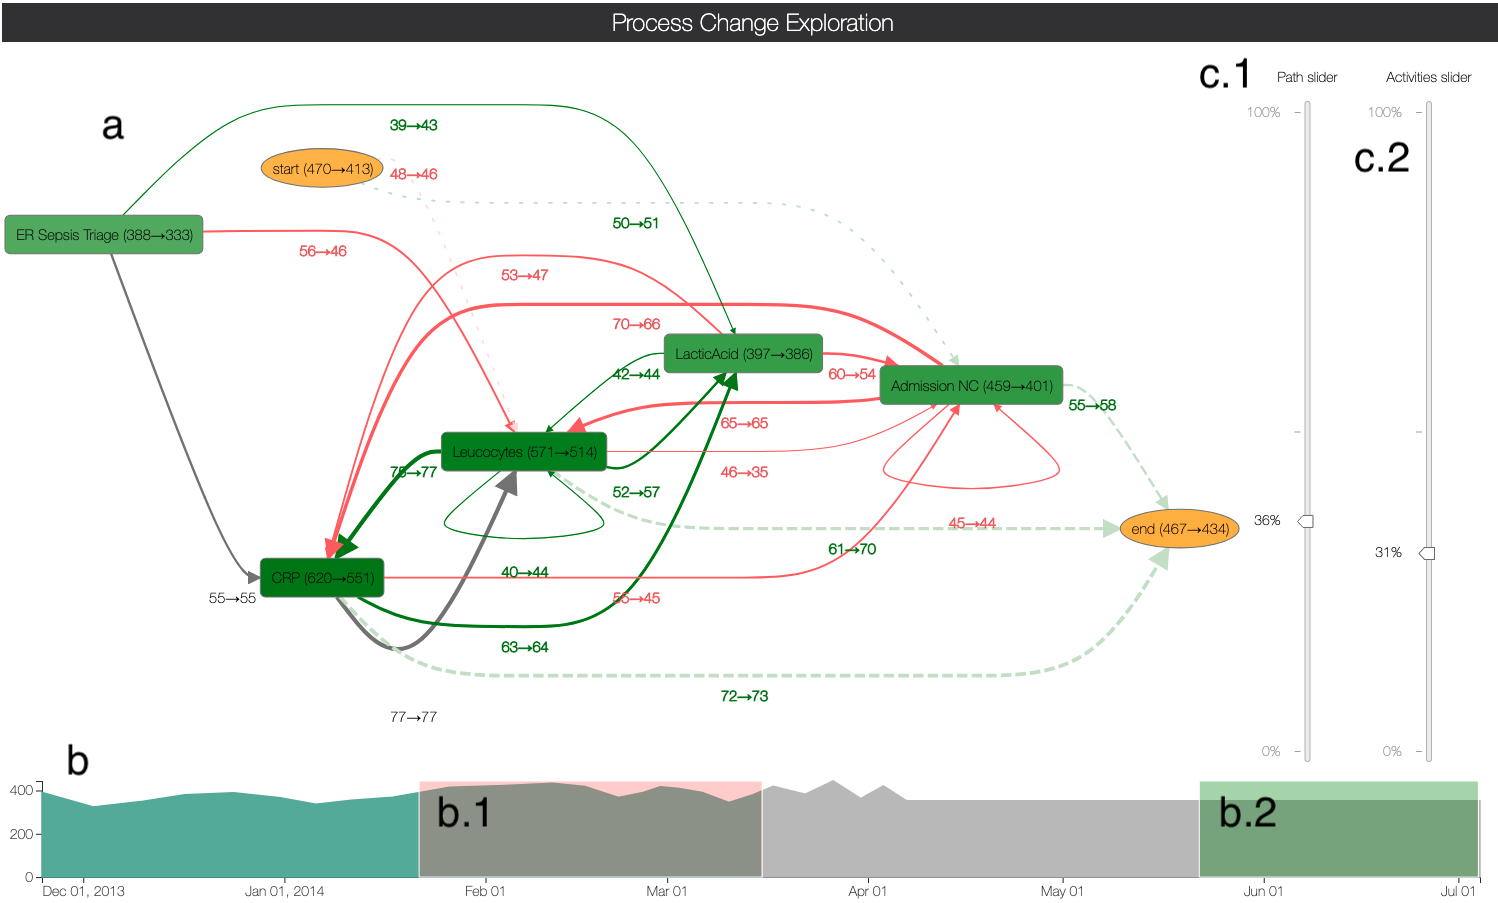
\includegraphics[width=\textwidth]{img/vis/vis-system-two-brushes.png}
	\caption{Process Change Exploration (PCE) system.~\emph{(b)} is the activity timeline view,~\emph{(a)} main Directly-follows graph view,~\emph{(c.1), (c.2)} additional filtering views.} 
	\label{fig:vis-two-brushes}
\end{figure}

%The interactive system consists of three parts. Part b shows the timeline of the data (green region), and forecasted values (grey region). The user can brush one or two regions (in this b.1 and b.2) on this graph to see the filtered for that time range process model or a difference between two process models. The main view (a) represents the directly follows change graph that shows the difference between two brushed regions. The c.1 and c.2 are the usual filters on the number of paths and activities to aid simplification the visual representation


The design of the PCE system is shown in Figure~\ref{fig:vis-two-brushes}. It shows an interactive visualization system with several connected views. The view~\emph{(b)} shows the area graph for the number of activities executed per each period. The green area represents the actual data, and the grey region represents the predicted values. Users can brush one or more regions on this graph in order to filter the scope of the analysis~\emph{(b.1}, and~\emph{b.2)}. If a user brushes two regions then the earlier will be color-coded in red, and the later color-coded in green. The main DFG view~\emph{(a)} is showing the directly follows graph of the brushed region when none or one region is selected or the difference between two brushed regions when two regions are brushed. In case the difference is showed, the red transitions are used to show the decrease in executions, green to show the increase and grey in case of stable behavior. For coloring, we used ideas from~\cite{DBLP:conf/grapp/KriglsteinR12}. Two additional views~\emph{(c.1)}, and~\emph{(c.2)} allow for the standard filtering~\cite{leemans2019directly} of activities and paths.

The process of designing and implementing the system started by designing several prototypes that undergone rounds of discussions to mature into the implemented visualization system. The system is implemented with D3.js JavaScript library and is available at~\footnote{\url{google.com}}.

%\begin{figure}
%	\centering
%	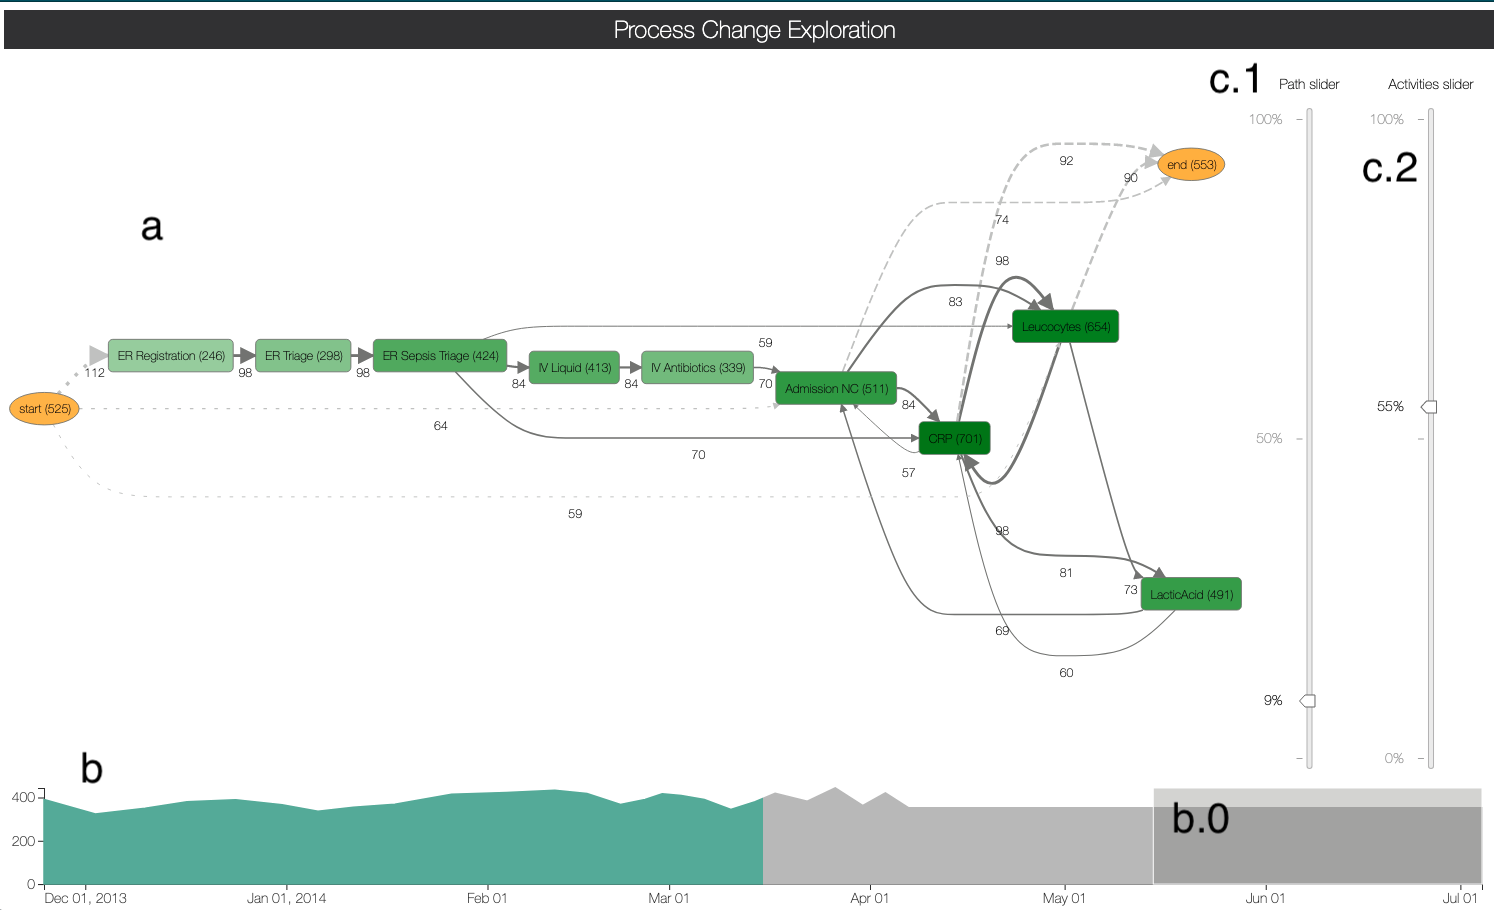
\includegraphics[width=\textwidth]{img/vis/vis-system-one-brush.png}
%	\caption{Process Change Exploration (PCE) system.} 
%	\label{fig:vis-one-brushes}
%\end{figure}

%Process Change Exploration (PCE) system. The interactive system consists of three parts. Part b shows the timeline of the data (green region), and forecasted values (grey region). The user can brush one time range (in this b.0) on this graph to see the filtered for that time range process model. The main view (a) represents the directly follows graph of that region. The c.1 and c.2 are the usual filters on the number of paths and activities to aid simplification the visual representation}

%
%\noindent\textbf{%
%Implementation. 
%} 


%\noindent\textbf{%
%	User interface
%} The Figure~\ref{fig:vis-two-brushes} displays the screenshot of the PCE visualization system. 
%We improve upon the notion of Directly-Follows graph~\cite{leemans2019directly} that is widely used in process mining research and practice. We use the ideas from the version graph~\cite{DBLP:conf/grapp/KriglsteinR12} on how to represent the change between versions of the graph with coloring of the transitions. 